\section{Design and Implementation}
\subsection{Approach}
The purpose of a network visualiser is to allow users to analyse and get insight into how they use the network\cite{Ruan2018}. It also allows network managers(advanced users) and researchers to schedule and perform measurements. The results of the measurements are also displayed on interactive graphs for further analysis.
\paragraph{}
For this project an iterative user-centred design(UCD) approach was adopted. This entails that the user is involved throughout the whole design process so that the visualisation produced meets every need that the user has\cite{Andrews:2006:EIV:1168149.1168151}. The goal of this approach is to find out the needs and tasks of the user and then design based on that\cite{Dylggduu}. This visualisation platform is developed for a system that is to be deployed at a local community network called iNethi in Cape Town. Users of this visualisation platform are expected to be network researchers, network managers and general users of the network.
\paragraph{}
This approach consisted of three phases:early envisioning phase, the global specification phase and the detailed specification phase\cite{Kulykinbook}.
\paragraph{}
The early envisioning phase entails the analysis of the users, the environment they are in and their tasks. This will enable us to profile users and gather requirements in the process\cite{Kulykinbook}. In the context of a network visualiser, the would mean understanding the type of data that user would to see visualised and analyse. A number of methods can be employed to obtain this which include surveys, interviews and focus groups\cite{Kulykinbook} \cite{Abras04user-centereddesign}.
\paragraph{}
In the global specification phase and the detailed phase, a designer comes up with a solution and presents it to users\cite{Abras04user-centereddesign} \cite{Kulykinbook}. Each phase may contain multiple iterations of design and analysis with evaluations taking place in all phases\cite{Abras04user-centereddesign}.
\paragraph{}
\begin{figure}[b]
	\centering
	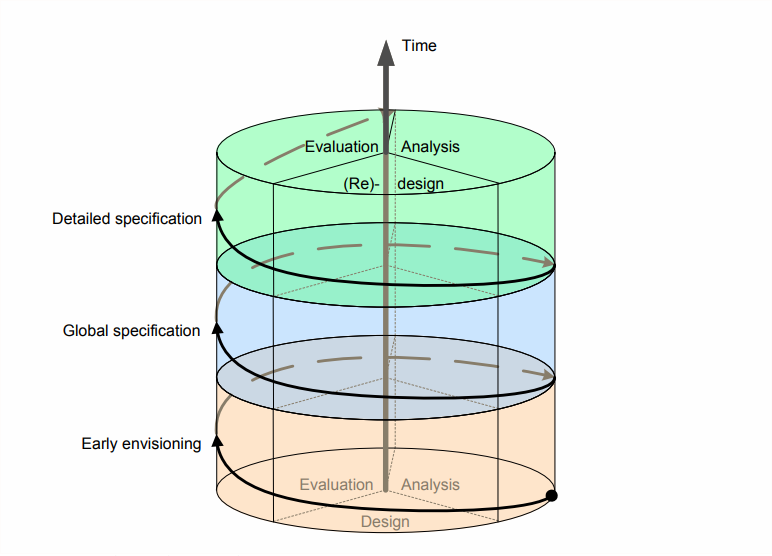
\includegraphics[width=0.7\linewidth]{img1}
	\caption{User-centered visualisation design process\cite{Abras04user-centereddesign}}
	\label{fig:img1}
\end{figure}

\paragraph{}
Users generally have different abilities and tasks to perform on the visualisation tool. Due to these differences it is imperative that a detailed analysis of the users, their environment and their tasks is performed before the design of the visualisation platform.

